\subsection{Leve1.2: 評価方法(目的関数の設計指針や方法)について}
\subsubsection{課題説明}
Amazonにおける書籍検索時に「ファンタジー作品で泣ける作品」を探し出すため
のアイテム集合$x$と目的関数$f(x)$について検討した。

% アイテム集合x: 目的関数に入力されるxは何か?
% 目的関数f(x): 入力されたxをどのように評価したら良いか?
% (オプション) 上記で設計した目的関数の欠点があれば例示と共に解説せよ。

\subsubsection{アイテム集合$x$について}
%私達のグループはhogeをfugaすることについて検討を進めた。すなわち云々

我々のグループでは,ファンタジー作品のレビューに書いてあるワードをアイテム集合$x$とすることを考えた.
次のようなレビューを例にとると,レビューに書いてあるすべての単語がアイテム集合$x$になる.
\begin{quote}
いやぁ、おもしろい。
異世界ファンタジーと言うのは、最初の数ページでこれはちょっと、と思う場合と、そこ
で引き込まれてあっという間と言う場合の二種類がある気がするけど、本書はもちろん後
者の方。
ありえなぁいと叫ぶだけのような、そんな浅いファンタジーではなく、とてもとても重厚
な、しっかり細部も練り込まれた、実に味わい深い作品でした。
\end{quote}

\subsubsection{目的関数について}
目的関数$f(x)$はすべてのアイテム集合$x$(レビュー内容の単語)に対して
重み付けをし,それを足し合わせた合計を返す関数とする.
先ほどのレビューを例にとると,「おもしろい」や「重厚な」,「味わい深い」などの作品を高く評価する単語に対しては
他のワードより大きな値を付加する.
そして探索目的は値が最大になるような$f(x)$である(図\ref{fig:level1-2}参照).

% (補足:PDF図を挿入する例)

\begin{figure}[h]
	\begin{center}
		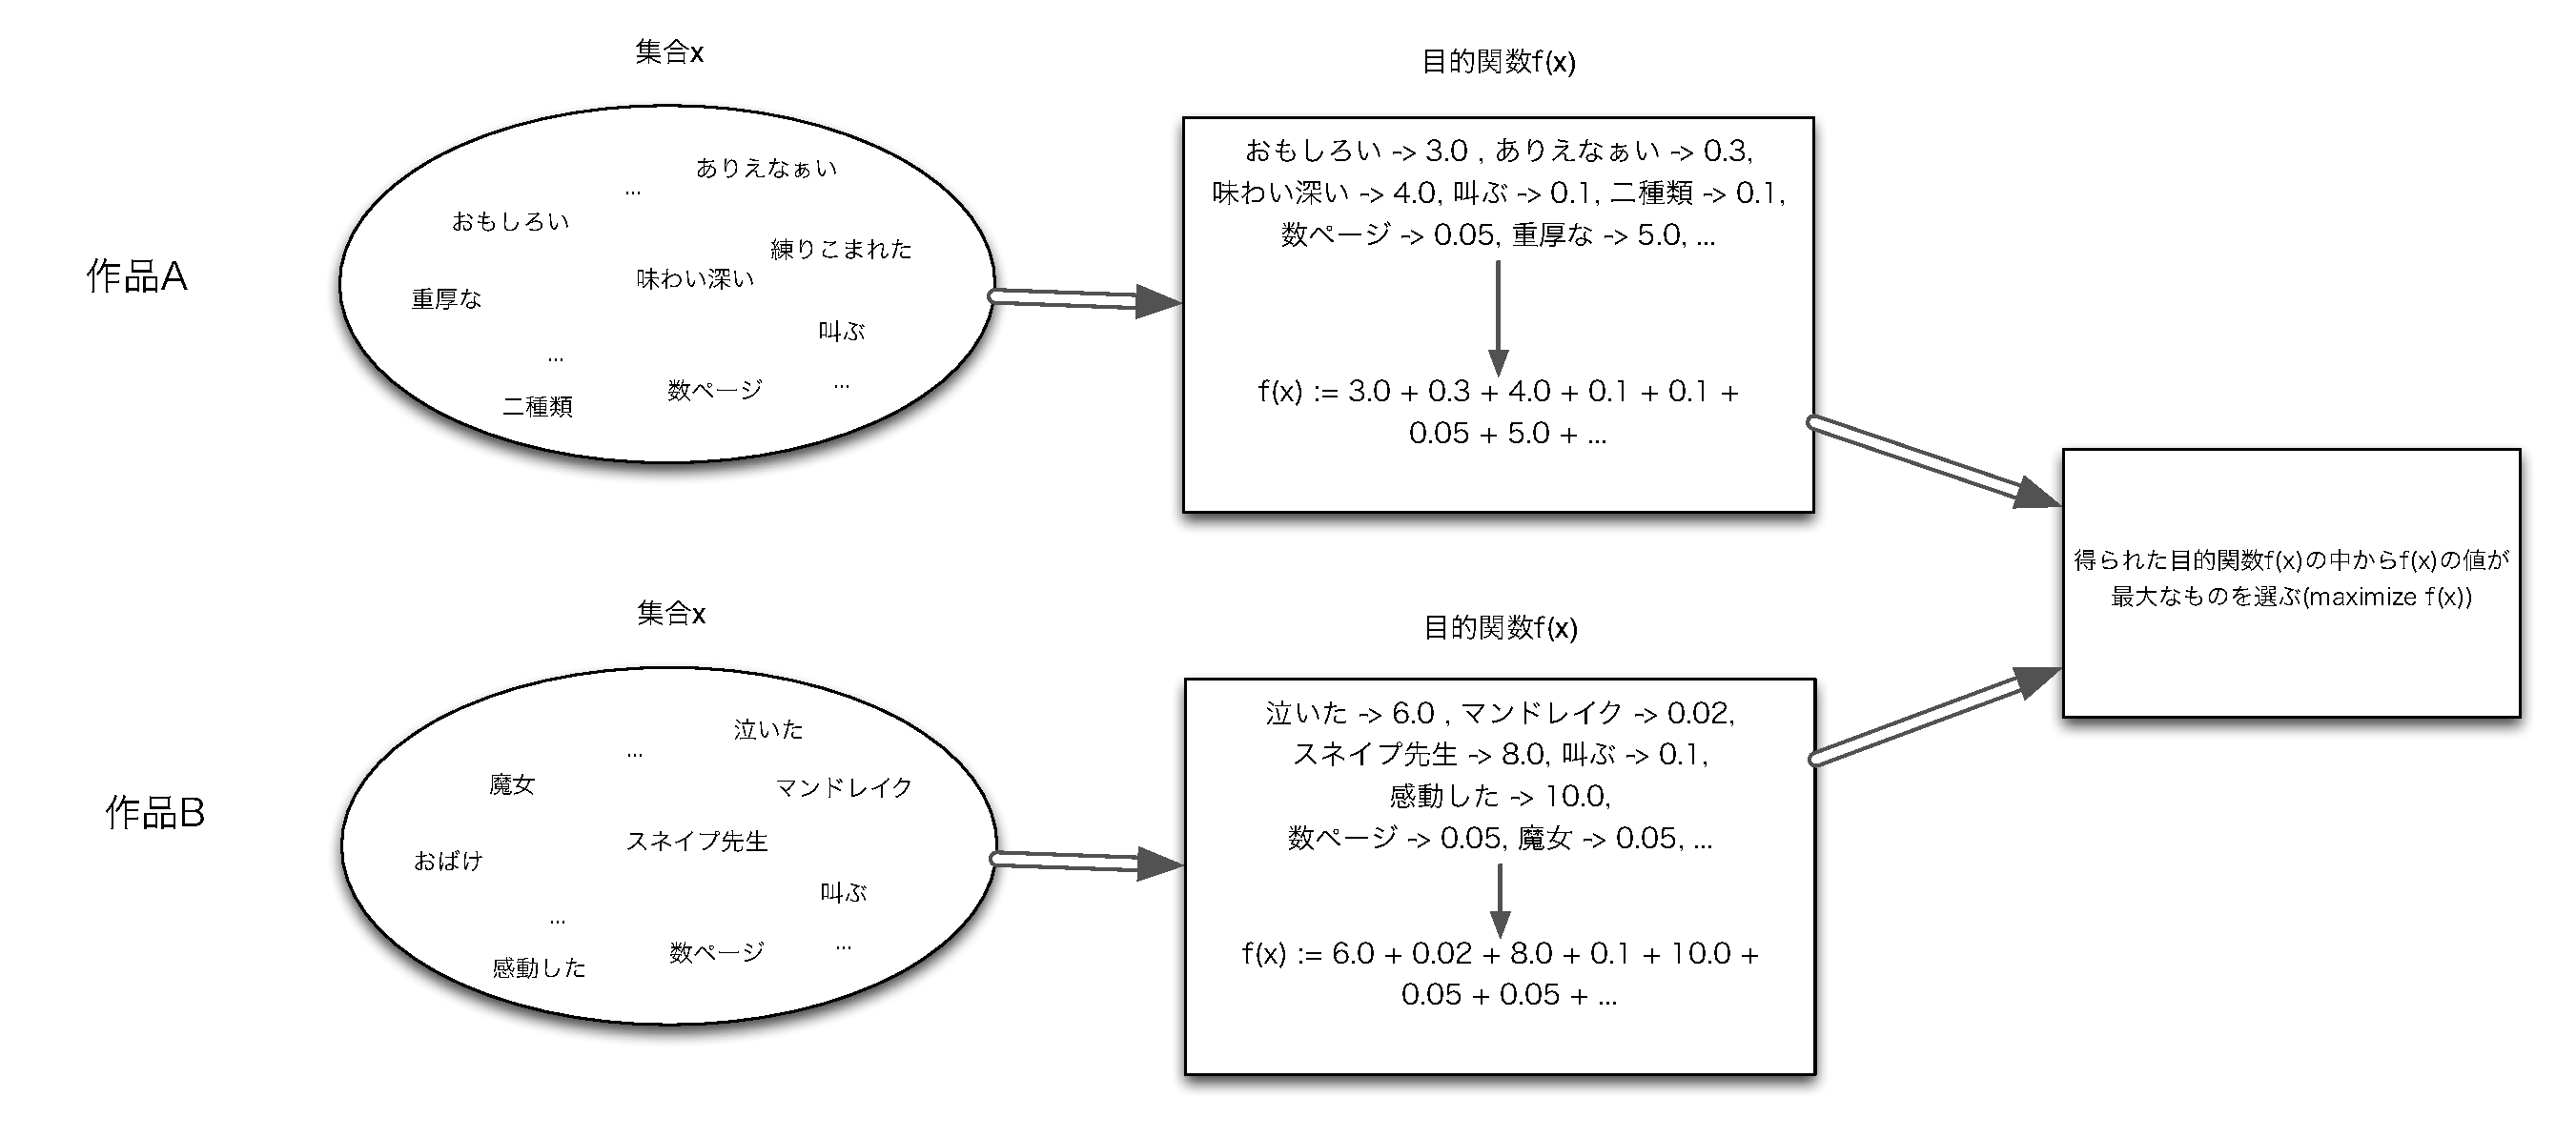
\includegraphics[scale=0.35]{./figs/level1-2.eps}
	\end{center}
	\caption{泣ける作品を探し出すまでの流れ}
	\label{fig:level1-2}
\end{figure}

\subsubsection{目的関数の欠点}
この目的関数の設計上の問題点は
あらかじめワードとワードに対応する重みの値を定義しておく必要があるということである.

